\documentclass{report}
\usepackage[utf8]{inputenc}
\usepackage{amsmath,amsfonts, amsthm, graphicx, geometry, lipsum}
\usepackage{hyperref}
\hypersetup{
    colorlinks=true,
    linkcolor=blue,
    urlcolor=red,
    pdftitle={How to write a thesis},
}

\usepackage{fancyvrb}
\usepackage{fancyhdr, lastpage}
\pagestyle{fancy}
\lhead{Trefor's awesome LaTex guide}
\rhead{Sponsored by Overlear!}
\cfoot{Page \thepage\ of \pageref{LastPage}}

\usepackage{etoolbox} %use carefully!
\patchcmd{\chapter}{\thispagestyle{plain}}{\thispagestyle{fancy}}


\begin{document}


\tableofcontents

\chapter{Useful Packages}

\section{Hyperref}
I want to link to my \href{https://youtube.com/drtreforbazett}{YouTube channel}.

\section{fancyvbr}

\begin{verbatim} [numbers=left, frame=single, formatcom=\color{red}]
    
    \begin{centre}
        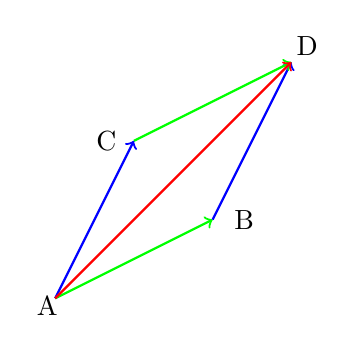
\begin{tikzpicture}
            
            \draw[thick, green, ->] (0,0) -- (2,1);
            \draw[thick, blue, ->] (2,1) -- (3,3);
            \draw[thick, green, ->] (1,2) -- (3,3);
            \draw[thick, blue, ->] (0,0) -- (1,2);
            \draw[thick, red, ->] (0,0) -- (3,3);

            \draw node at (-0.1, -0.1) {A};
            \draw node at (2.4, 1) {B};
            \draw node at (0.65, 2) {C};
            \draw node at (3.2, 3.2) {D};
            
        \end{tikzpicture}
    \end{centre}
    
\end{verbatim}



\section{fncyhdr}

\section{etoolbox}

\section{GitHub}

\section{fncychap}

\section{Color}

\section{Tcolorbox}

\section{SI units}

\section{Setspace}

\section{Glossaries and Acronyms}




\end{document}
